With the high level design and primary component selection complete, schematic capture and PCB layout of the VNA could begin. KiCad was used for all steps of the PCB design process, as it is a powerful free and open source EDA tool which is extensively used in the open source hardware community. For firmware, System Workbench for STM32 was utilised, as it provides open source tools such as GCC for Cortex-M cross compiling, OpenOCD for programming and debugging, precompiled and integrated in an Eclipse IDE, which makes getting firmware development started with a completely open source flow easy.

\subsection{Schematic Capture}
The first step in PCB design is schematic capture, where abstract representations of the components are joined together in a way which makes it easy to read and determine the desired functionality of the device. Due to development boards being designed earlier in the process, certain components such at the MAX2871 PLL, filter bank, and gain control circuitry were easily ported over into the new schematic, however due to issues such as a new amplifier needing to be designed in, along with the programmable attenuator being out of stock, changes were required to ensure that all components were able to be sourced in time, along with preforming as desired.

Other components such as the STM32 microcontroller, dual directional couplers, numerous status LEDs, and an auxiliary USB connection for powering DUTs and ECal units were also added to ensure that all required hardware was on device. Additionally numerous design for test additions such as 0 ohm resistors and DNP components, test points on all key signals, additional components in the PLL loop filter to allow an alternative PLL to be utilised, user addressable LEDs, unused pints being broken out, power rail LEDs, numerous ground points along with a unused UART connection were all designed in to make bring-up of the board as easy as possible. The completed schematic can be found in Appendix \ref{appen:vna_design_files}, Figures \ref{fig:vna_schematic_overview} through \ref{fig:vna_schematic_power}.

\subsection{Layout Planning}
Before PCB layout can begin, there are a few key steps and decisions which need to made which will place constraints on the design of the PCB. Firstly, component footprints were associated with the relevant schematic symbols, with footprints being designed where KiCad did not have them in the standard library. Furthermore 3D models for every component were either loaded from KiCad, sourced from the distributor, or drawn from mechanical drawings, as this would allow for mechanical fit with an enclosure to be confirmed later in the design process. 

With all the components imported into CAD, the approximate size of the PCB was able to be determined. This allowed for COTS aluminium case options to be explored, and once an enclosure was found which was large enough for the PCB to fit, the exact dimensions of the PCB were able to be fixed to that dimension, allowing the positioning of connectors, mounting holes, and other key features of the PCB to be placed. 

The PCB stackup and manufacturer also needed to be determined, as this plays a key role in the cost of the boards, along with key PCB features such as minimum space / trace, via size, and the width of a 50 ohm microstrip trace. Due to cost and prior experience, JLCPCB was chosen as the manufacturer, and their 4 layer FR4 "JLC7628" stackup (Table \ref{table:pcb_stackup}) was chosen as it is a very common stackup well suited to the feature and component sizes used on the board, along with the ability for it to be ordered from other manufacturers with ease. Furthermore, a Signal / GND / PWR / Signal configuration would be designed for during layout, with additional flood fills of ground on layers 1 and 4. 

\begin{table}[H]
	\centering
	\caption{Chosen PCB stackup}
	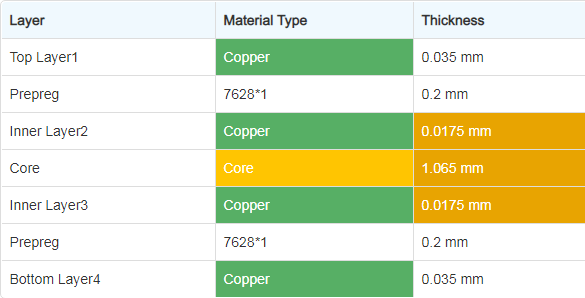
\includegraphics[width=0.8\linewidth]{jlc_stackup.png}
	\label{table:pcb_stackup}
\end{table}

Other key feature sizes for the chosen stackup and manufacturing process are outlined in Table \ref{table:pcb_specs}. It should be noted that whilst JLCPCB are able to do quite small trace / space and via drill size, 6/6 trace/space and 0.25/0.5 drill/via were chosen for the design, as this would allow it to be fabricated at common fabricators such as OSHPark and PCBWay without paying for advanced processes. 
\begin{table}[H]
	\caption{Key specifications of PCB design rules and feature size}
	\label{table:pcb_specs}
	\centering
	\begin{tabular}{|c|c|}
		\hline
		\textbf{Feature}                          & \textbf{Dimension} \\ \hline
		Min Trace / Space                         & 0.15 mm (6 mil)   \\ \hline
		Min Via Drill Size                        & 0.25 mm (10 mil)     \\ \hline
		Min Via Diameter                          & 0.5 mm (20 mil)   \\ \hline
		50 $\Omega$ Microstrip Width              & 0.29 mm (11.5 mil) \\ \hline
		Blind / Buried / Micro Via                & Not Available \\ \hline
	\end{tabular}
\end{table} 

\subsection{PCB Layout}
Given the mechanical dimensions, stackup, and design rules have be determined, these parameters can be loaded into KiCad and the PCB can be laid out. An image of the laid out board can be found in Figure \ref{fig:pcb_layout}, with an image of the assembled board available in Figure \ref{fig:pcb_render}.

Given the operating frequencies seen on the board, a number of key layout considerations were taken into account to ensure optimal function of the board, and are detailed below.
\begin{itemize}
	\item \textbf{50 $\Omega$ RF Traces} need to be kept along the signal path to ensure a good match between components, and this is achieved on this board through using a 0.29 mm microstrip on layer 1 over a continuous ground pour on layer 2. 
	\begin{itemize}
		\item Furthermore, compensation for extra capacitance introduced under the large pads of the directional couplers and SMA connectors need to occur, as otherwise there will be added capacitance which will decrease the match of the transmission line. This can be seen in Figure \ref{fig:pcb_cap_comp}, where the ground fill has been removed to significantly reduce the inter-planar capacitance between layers 1 and 2, to ensure a consistent characteristic impedance. 
		\item When a layer change is required for the RF signal, care must be taken to ensure there is a low impedance path between reference layers. This can be seen on the first directional coupler as shown in Figure \ref{fig:pcb_layer_change}, where the RF travels from the bottom left on layer 1, through a via to layer 4, and back to layer 1 in the top right hand corner. Stitching vias can be seen close to the signal via to ensure a low inductance path between the two reference planes, along with the signal vias being optimised to have a 50 $\Omega$ impedance to reduce impedance discontinuity. 
		
		Unfortunately a mistake was made during layout in that the signal was routed on layer 4 instead of 3, as with the signal on 4 its reference plane is layer 3, VCC, which does not have a low inductance path to layer 2, as the closest decoupling capacitor is located in the top left of the figure, near the 8 pin DFN IC. Ideally the signal would have been routed on layer 3,  allowing the ground pour on layer 4 to be the reference plane, with the multiple vias providing a low inductance path between the two planes. Fortunately, due to upper bounds of the frequencies seen on the board at 1.25 GHz, this is not a major issue which has caused issues with the function of the device. 
		\item Low impedance between layers was also ensured through the use of ample stitching vias, both around the signal path and the entire board. 
	\end{itemize} 
	\item \textbf{Power Integrity} was achieved through the use of linear regulators to decrease noise on the power rails, low inductance connections to components through large power planes, and multiple vias when changing layers to ensure the added inductance is kept to a minimum. Furthermore, ensuring the decoupling capacitors specified in application notes for each component are placed close the power pins, with the smaller capacitors closer to the pin, and a dedicated via for each capacitor placed as close as possible to the pad ensures that the impedance and noise seen at the power pin to each component is kept at a minimum, which leads to optimum performance of the IC and minimal coupling of noise onto the RF and analog signals.
	\item \textbf{Following reference layouts} ensured that the device would preform as specified on the data sheet, along with being able to rule out bad component placement and routing as possible causes for improper function of device. Where reference designs were not available, best RF layout practices including those described above were utilised to ensure optimal performance of the device.  
\end{itemize} 

\begin{figure}[H]
	\centering
	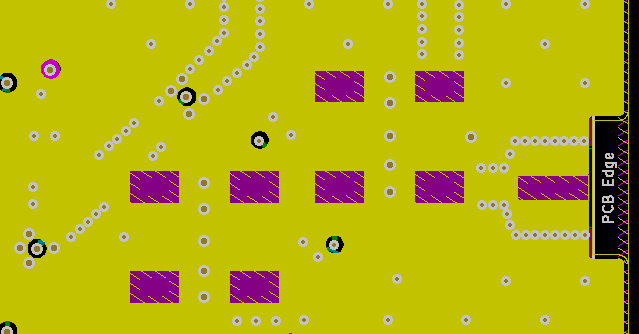
\includegraphics[width=0.7\linewidth]{ground_cutouts.png}
	\caption{Ground cut-outs under large pads to reduce inter-planar capacitance and ensure a 50 $\Omega$ transition}
	\label{fig:pcb_cap_comp}
\end{figure}

\begin{landscape}
	\begin{figure}
		\centering
		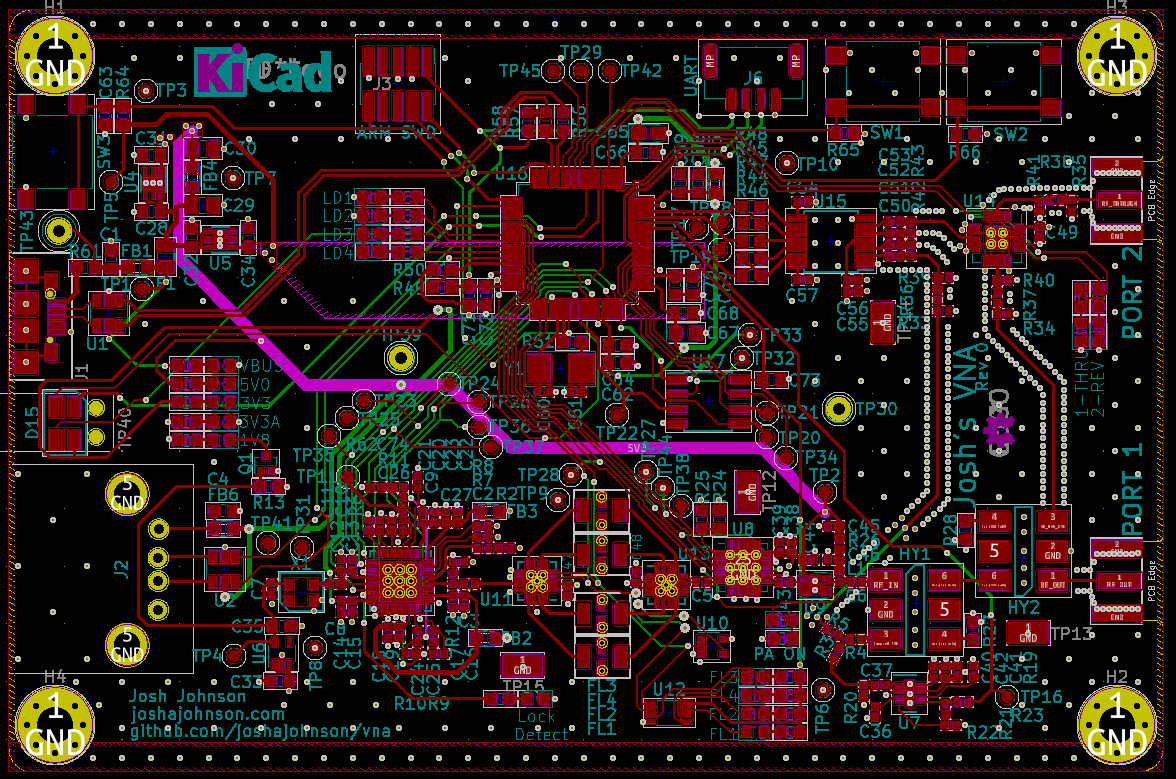
\includegraphics[width=\linewidth]{pcb_layout.png}
		\caption{PCB Layout, with Red = Layer 1, Yellow = Layer 2, Pink = Layer 3, Green = Layer 4. Flood fill of each layer is not shown.}
		\label{fig:pcb_layout}
	\end{figure}
\end{landscape}

\begin{figure}[H]
	\centering
	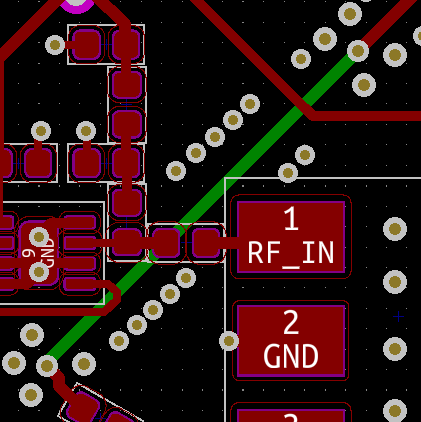
\includegraphics[width=0.35\linewidth]{layer_change.png}
	\caption{Layer change mistake on the signal path}
	\label{fig:pcb_layer_change}
\end{figure}

\subsection{Mechanical Design}
To ensure there will be no mechanical clearance issues, a 3D model of the board was exported from KiCad into Fusion360 and placed into a model of the extrusion, and it was seen that there were no mechanical issues. Having the 3D model in MCAD, together with the decision to use an extruded aluminium enclosure results in easy design of custom front and rear panels, as key features from the 3D model can be referenced when designing cut-outs for the connectors and light pipe. DXFs were exported from Fusion360 back into KiCad where they had silkscreen added, and they were then sent off to be manufactured with the main VNA PCB. Renders of the front and rear panels can be found in Figures \ref{fig:pcb_front_render} and \ref{fig:pcb_rear_render}, and the assembled VNA without the top extruded section in Figure \ref{fig:pcb_assembled}.

\begin{figure}[H]
	\centering
	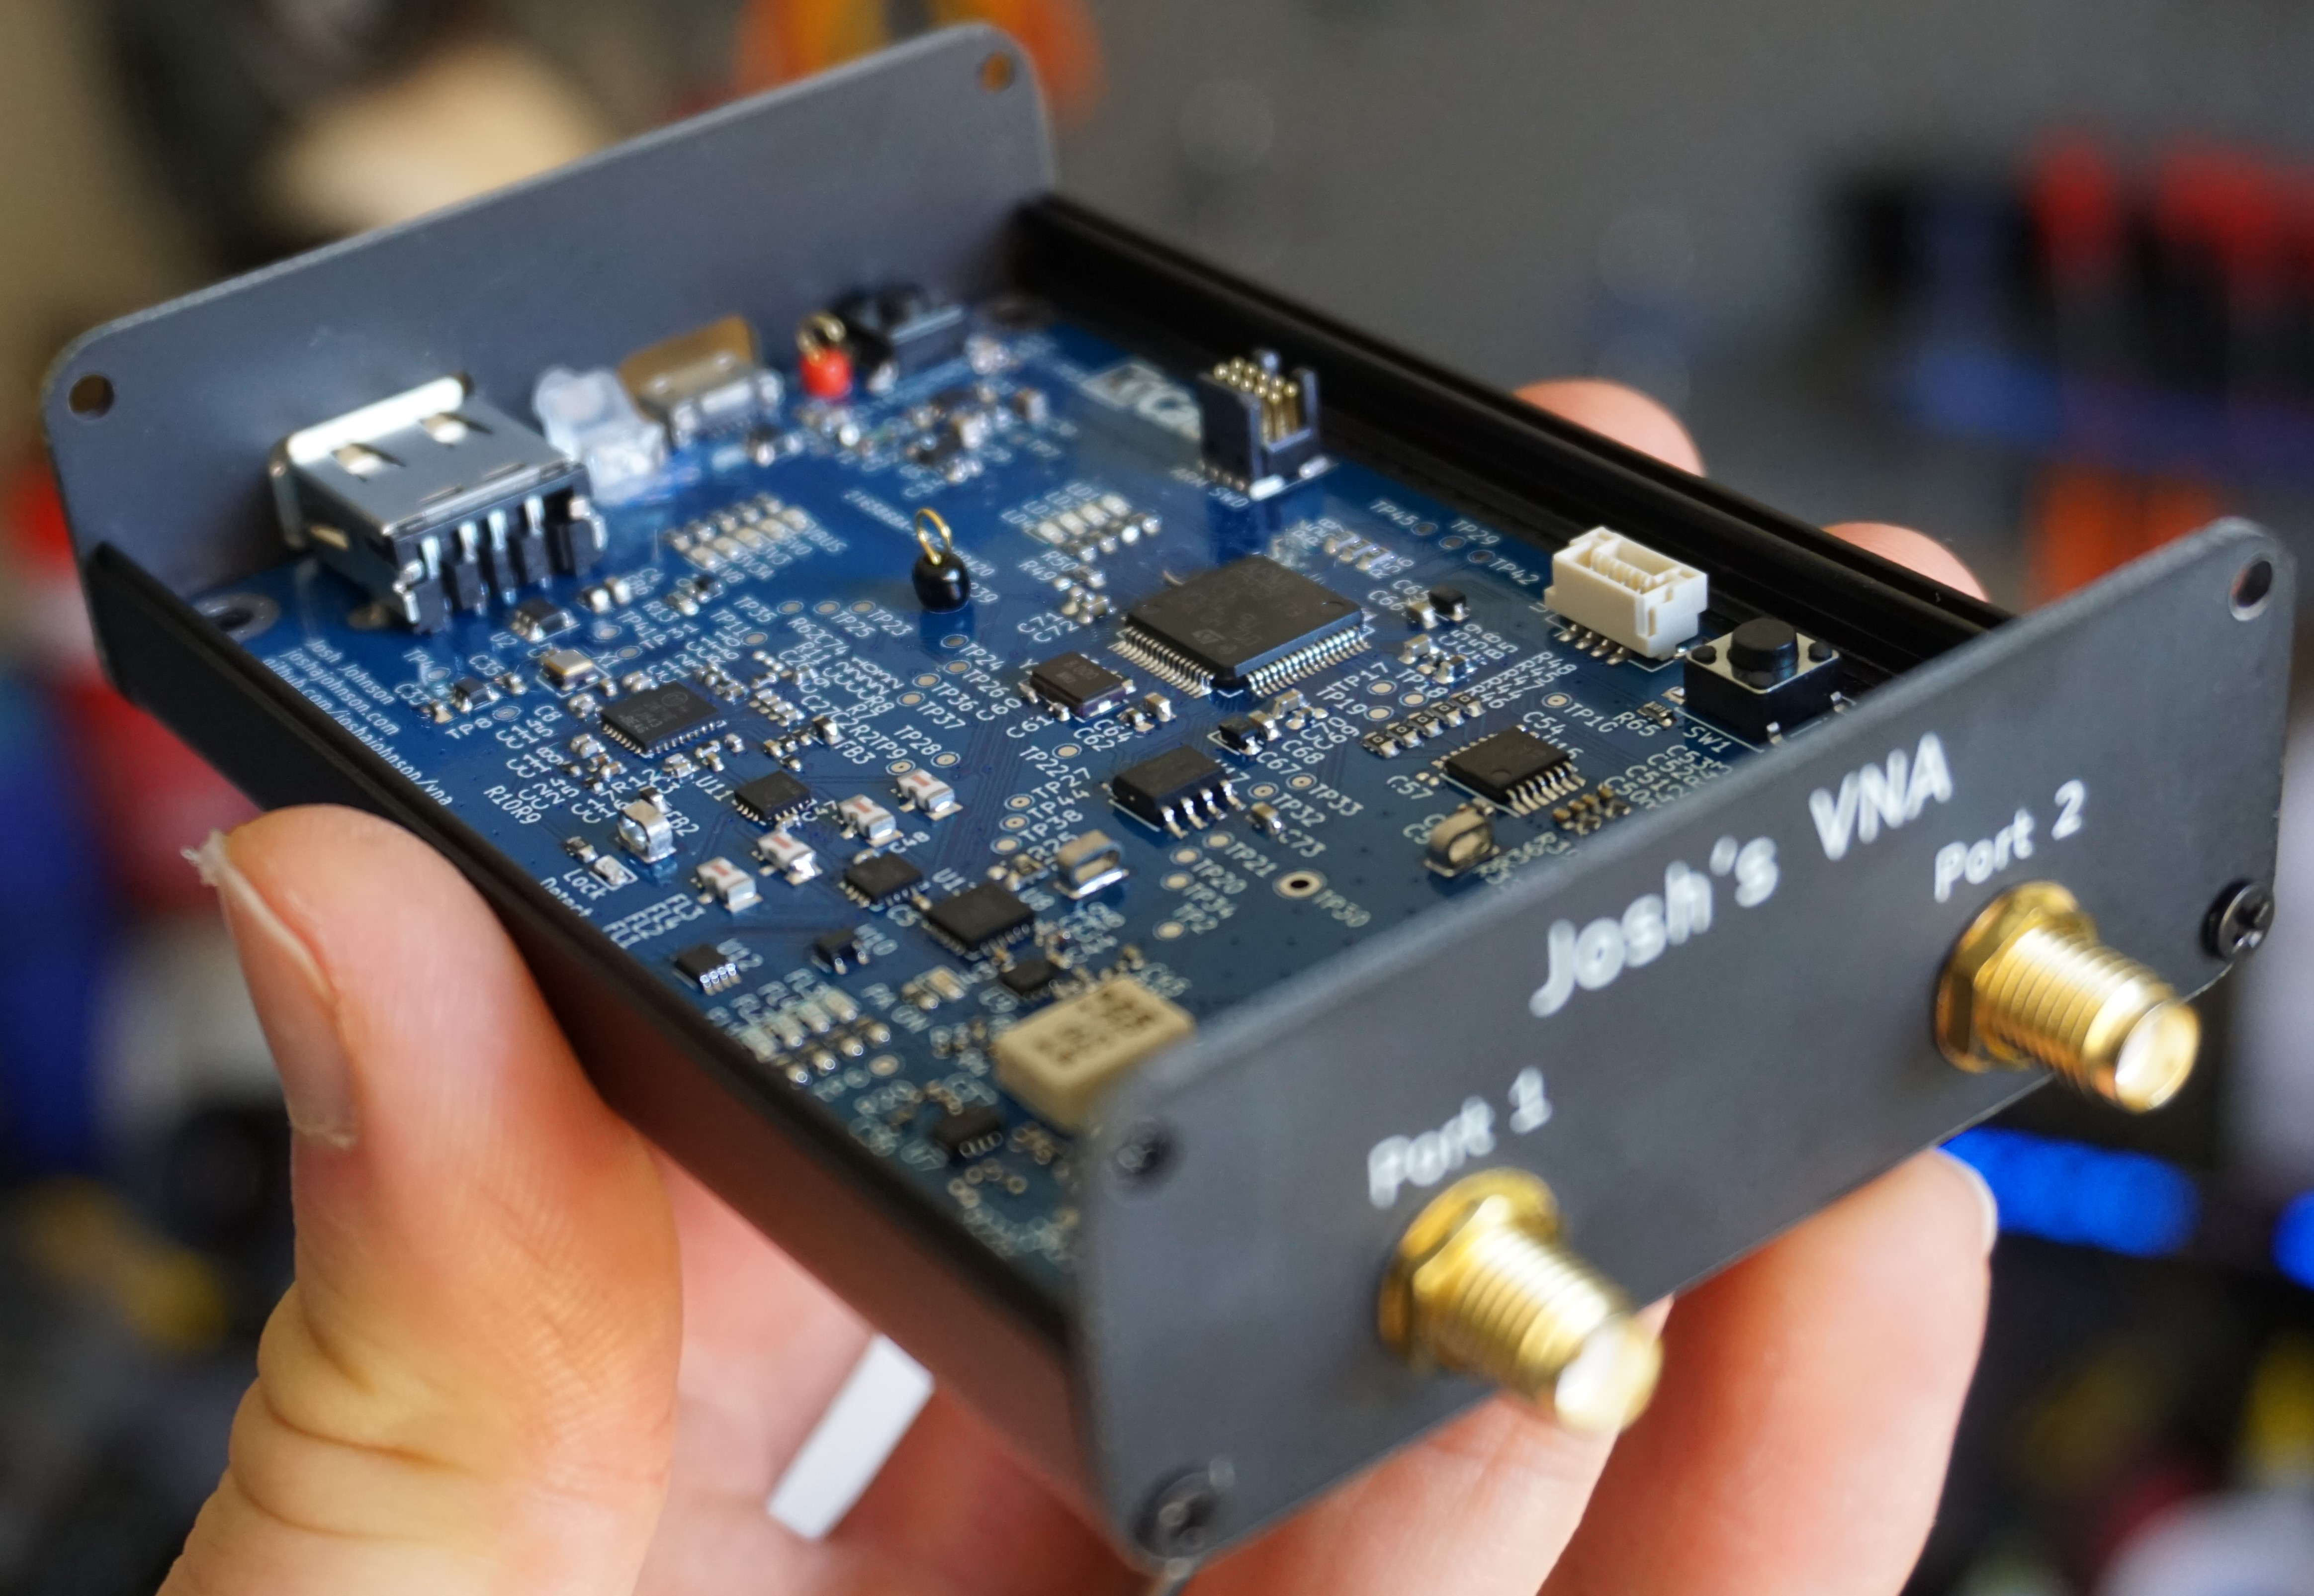
\includegraphics[width=0.7\linewidth]{assembledVNA.jpg}
	\caption{Assembled VNA in enclosure, with top section removed}
	\label{fig:pcb_assembled}
\end{figure}

\subsection{Assembly + Bill of Materials}
Upon arrival of the PCBs and solder paste stencil, assembly was undertaken. This followed a fairly standard SMT process, with solder paste being deposited onto the PCB through the use of a stencil, placement of components under a microscope due to their size (down to 0402 and 0.5 mm QFN), and reflow in a reflow oven. Rework was required for a few components due to tomb stoning, along with some shorted pins on the QFNs, along with hand soldering of the through hole components and SMA connectors. The board was then cleaned in an ultrasonic cleaner to remove any remaining flux, and left to dry for an hour in the reflow oven. This process went quite smoothly with the whole process taking less than 6 hours from start to finish. 

Table \ref{table:BOM} outlines the cost to manufacture one VNA, with removal of components such as debug headers and ground test points which are only required on the development boards. As can be seen, the cost for one VNA comes out to \$272.88, including the full cost of 5 PCBs and the enclosure. It should be noted that the per board cost at quantity 10 is reduced to \$204.78 due to the cost of PCBs being split between multiple boards and a slight reduction in component price, and that if free samples are requested from Analog Devices and Maxim and no case is utilised, the cost of assembling a VNA can be as little as \$185.37. Pricing is correct as of 10/10/19.

\subsection{Board Errata}
There were a few issues found during board bring-up which required hardware changes. Firstly, buttons which were placed on device to aide debugging were drawn up incorrectly in the schematic and resulted in both sides of the button being tied to ground. This was resolved by lifting pads of the button and connecting them to 3V3 as required.

A more challenging issue to resolve was found in that upon reset of the microcontroller, it would not re-enumerate with the host however Windows would still show it as connected. Following some googling it was found that Windows requires the 1K5 pull-up resistor on D+ to be pulled to ground during reset, as this triggers re-enumeration of the device. This issue was resolved by connecting the pull-up resistor to an unused GPIO pin which upon start-up would pull the pin low, wait a few milliseconds, and then assert it high to force re-enumeration. 

The only other hardware issue found on the board was to do with the configuration of the MAX2871's output signals. Upon bring-up of the transmit chain, it was noted that the RF power was far too low and this was narrowed down to the output of the MAX2871 being tens of dB below the expected output power. The issue was found to be incorrect termination of the unused RF- output to ground through a 50$\Omega$ resistor, instead of being pulled up to 3V3 through a resistor before being tied to ground. This was resolved with reworking some 0402 components and adding a flying wire as shown in Figure \ref{fig:max_rework}.

\begin{table}[h!]
	\caption{Bill of Materials for VNA}
	\label{table:BOM}
	\centering
	\begin{tabular}{|c|c|c|c|c|}
		\hline
		\textbf{Quantity} & \textbf{Part Number}       & \textbf{Description}     & \textbf{\begin{tabular}[c]{@{}c@{}}Price Each \\ (\$AUD)\end{tabular}} & \textbf{\begin{tabular}[c]{@{}c@{}}Per Board \\ (\$AUD)\end{tabular}} \\ \hline
		1                 & MAX2871                    & PLL with VCO             & 18.95                                                                 & 18.95                                                                     \\ \hline
		1                 & ASTXR-12         & Reference Clock          & 4.75                                                                  & 4.75                                                                      \\ \hline
		2                 & PE42440                    & SP4T Switch              & 1.93                                                                  & 3.87                                                                      \\ \hline
		1                 & LFCN-105+                  & Low Pass Filter          & 15.27                                                                 & 15.27                                                                     \\ \hline
		1                 & LFCN-225+                  & Low Pass Filter          & 11.45                                                                 & 11.45                                                                     \\ \hline
		1                 & LFCN-400+                  & Low Pass Filter          & 11.45                                                                 & 11.45                                                                     \\ \hline
		1                 & LFCN-1000+                 & Low Pass Filter          & 7.61                                                                  & 7.61                                                                      \\ \hline
		1                 & TRF37A75                   & Power Amplifier          & 2.84                                                                  & 2.83                                                                      \\ \hline
		1                 & SKY12347-362LF             & Attenuator  & 10.04                                                                 & 10.04                                                                     \\ \hline
		2                 & ADC-15-4+                  & Directional Coupler      & 19.21                                                                 & 38.43                                                                     \\ \hline
		1                 & AD8319                     & Log Power Detector       & 8.69                                                                   & 8.69                                                                       \\ \hline
		1                 & AD8302                     & Gain Phase Detector      & 45.10                                                                   & 45.10                                                                       \\ \hline
		1                 & F2923                      & SPDT RF Switch           & 8.20                                                                  & 8.20                                                                      \\ \hline
		2                 & SMA                        & DUT Connector            & 2.12                                                                  & 4.24                                                                      \\ \hline
		1                 & Micro USB                  & Connection to PC         & 0.12                                                                  & 0.12                                                                      \\ \hline
		1                 & USB A                      & External Connection & 0.42                                                                  & 0.42                                                                     \\ \hline
		2                 & LP5912                     & 3V3 LDO                  & 2.01                                                                 & 4.02                                                                     \\ \hline
		1                 & MIC5366-1.8                & 1V8 LDO                  & 0.37                                                                  & 0.37                                                                      \\ \hline
		1                 & Polyfuse                   & Input protection   & 0.39                                                                  & 0.39                                                                      \\ \hline
		2                 & TPD2S017                   & ESD Protection           & 1.05                                                                  & 2.11                                                                      \\ \hline
		1                 & STM32F373              & Microcontroller           & 8.87                                                                 & 8.87                                                                      \\ \hline
		1                 & 8 MHz Crystal              & For MCU                  & 0.83                                                                  & 0.83                                                                      \\ \hline
		1                 & RGB LED                    & Status LED               & 0.88                                                                  & 0.88                                                                      \\ \hline
		1                 & Assorted Capacitors        &                          & 2.20                                                                    & 2.20                                                                        \\ \hline
		1                 & Assorted Passives &                          & 1.10                                                                    & 1.10                                                                        \\ \hline
		1                 & VNA PCB                    & (Price for 5)            & 45.67                                                                 & 45.67                                                                     \\ \hline
		1                 & Enclosure                  &                          & 8.28                                                                  & 8.22                                                                      \\ \hline
		2                 & Front/Rear Panels         & (Price for 5)            & 3.26                                                                  & 6.53                                                                      \\ \hline
		1                 & Light Pipe                 &                          & 0.98                                                                   & 0.98                                                                       \\ \hline
		&                            &                          &                                                                        &                                                                            \\ \hline
		&                            &                          & Total Cost                                                             & 272.88                                                                    \\ \hline
	\end{tabular}
\end{table} 

\newpage
\subsection{ECal Design}
To aide with use of the VNA, a low cost ECal unit was designed which switches in calibrations standards based on commands from the VNA. It is controlled through the use of a USB cable, where the data pins are either I2C so a port expander with up to 16 control pins can be utilised, or GPIO, so a SP4T switch can be controlled by toggling two pins. Furthermore, the design utilises a two layer board with a grounded coplanar waveguide for the RF trace, as the trace width required on a 1.6mm substrate for a 50$\Omega$ transmission line is far too wide for easy design and would result in increased impedance mismatch during tapering of the trace to meet the 0.3mm pads of the QFN switch. 

For the ECal to be utilised, it's S-parameters must be measured with a VNA as this effectively transfers the calibration from the VNA's calibration standards to the ECal unit, and from there the ECal's generated touchstone file can be used as a reference of the expected frequency response. Unfortunately due to the VNA accessed at ANU not having a SMA calibration kit the ECal was not able to be measured and as such used during development, but it has been shown to function and as such if it was measured there is nothing stopping it from being used as a substitute for discrete calibration standards.

The schematic for the RF section of the VNA can be found in Figure \ref{fig:ecal_schematic}, with an image of the assembled unit in Figure \ref{fig:ecal_photo}.

\begin{figure}[H]
	\centering
	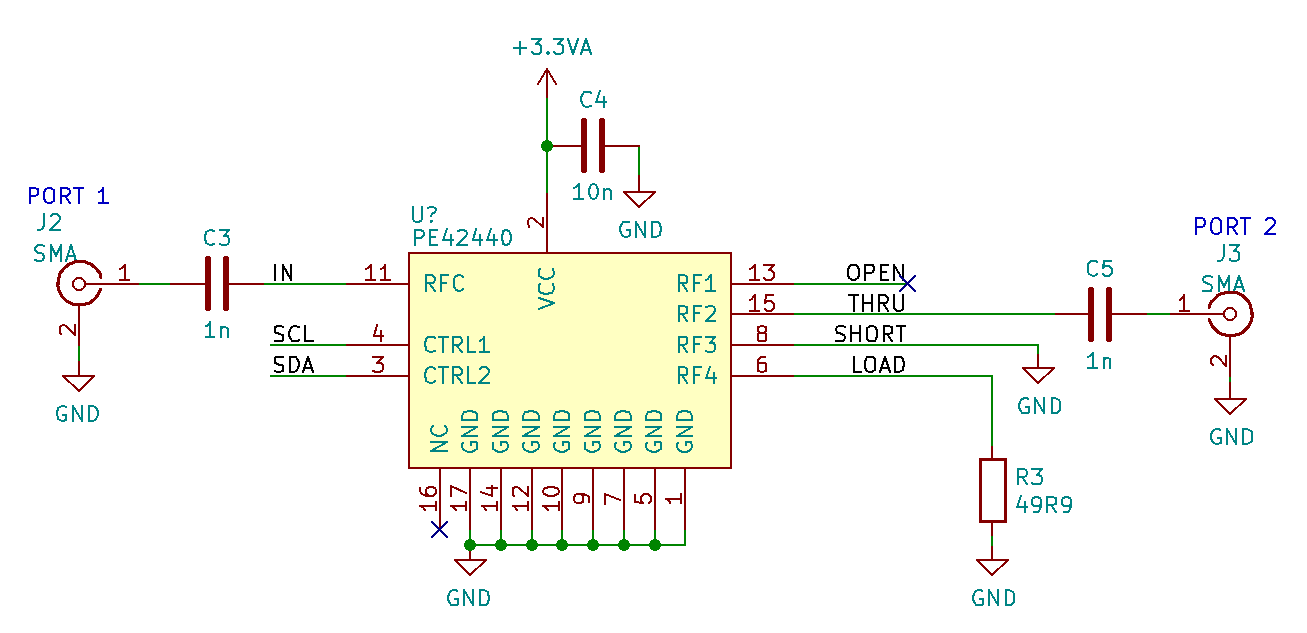
\includegraphics[width=\linewidth]{ecal_schematic.png}
	\caption{Schematic of the ECal RF circuit}
	\label{fig:ecal_schematic}
\end{figure}

\newpage
\subsection{Firmware Development}
Firmware development for the STM32F373 was done in C, with the use of ST's Hardware Abstraction Library (HAL) configured through STM32CubeMX which allowed easy configuration and interaction with the onboard peripherals. An Eclipse based IDE, along with numerous programmers / debuggers were used for development and debugging of the firmware, which was complied with GCC to meet the requirement for an open source toolchain. As outlined in Figure \ref{fig:sw_flowchart}, there are numerous steps required to receive, process, command, measure, and return the required information for function of the VNA, and the firmware blocks developed for each of these steps will be discussed below, along with some of the challenges overcome during development. 

\subsubsection{Start-up and Initialisation}
Upon start-up, initialisation of a number of peripherals is required. Along with configuring the GPIO, SPI bus, timers, and USB peripherals, the ADC is initialised and calibrated, which results in reducing the offset and gain errors through an internal alignment process \cite{st_sdadc}. The pull-up on USB D+ is also cycled, as this forces re-enumeration of the device if the VNA had undergone a warm reset. 

\subsubsection{USB and Command Parsing}
A virtual COM port is used for communicating with the host computer, as due to the low data rates required and the universal compatibility of a COM port it is well suited to the task. ST's HAL provides a function which is called from an interrupt every time a character is received, however the implementation of code which handles the received data is left to the user. As such, a circular buffer was implemented which allows for receiving data, along with error checking and warnings to be sent over serial and indicated on the onboard status LED if the buffer becomes overrun or an unexpected error occurs. A function \texttt{scanUSB} was implemented to wait for a completed transmission from the COM port, and move the received characters into a null terminator padded string which would allow other sections of the code to parse the string without concern for it's location in the circular buffer. 

A command parser was also written which splits the received string into commands and arguments based upon defined delimiters, and then using a lookup table finds the intended function and calls it with the passed arguments. Minimal error checking is done at this stage, as it is expected that either the user or Python script which calls the function is passing correct values, and if any bad variables are passed the low level hardware control code will catch the issue. 

Along with the \texttt{measure} command which measures S-parameters, the VNA can also be commanded to act as a signal generator, sweep frequencies, configure the ECal unit, along with low level control such as configuring the output filter used, level of attenuation, enabling / disabling the PA and LO, along with reporting the status of various settings which was not only helpful during development but can be used to demonstrate the internal function for educational purposes. 

\subsubsection{Measurement Control}
When the user chooses to measure S-parameters, they pass in which parameter (S\textsubscript{11}, S\textsubscript{21}), start and stop frequency, number of steps, along with the output power level to be held throughout. From this, there are a number of steps which occur:
\begin{itemize}
	\item To indicate that the VNA is working, it illuminates a status LED blue before beginning measurement.
	\item The input switch is configured to either allow the reflected or transmitted RF to pass through to the AD8302 gain / phase detector. 
	\item The AD8302 VREF is read, as it will be used later on to remove any offset between the AD8302 and ADCs in the STM32.
	\item The required frequency step is determined, and a while loop is entered which preforms the following functions, whose workings will be described below:
	\begin{itemize}
		\item The transmit chain is configured to have the correct frequency, filters, and output power level. 
		\item The AD8302 is sampled numerous times and returns averaged voltages corresponding to the gain and phase measurements. 
		\item Conversion is then done to convert the raw voltages into gain and phase values in dB and degrees respectively, which includes the first step in phase correction. 
		\item The frequency, gain, and phase measurements are then sent over serial to the host computer, before incrementing the frequency. 
	\end{itemize}
	\item Once all required frequencies have been measured, the VNA turns its status LED green to indicate it is finished, and waits for a new command. 
\end{itemize}

\newpage
\subsubsection{Transmit Chain Configuration}
Transmit chain configuration begins with the MAX2871 PLL, which was the single most challenging part of the project, as it has six 32 bit registers which all need to be configured correctly for function, however the data sheet is light on detail and there is no application note detailing configuration of it. Maxim do however provide a tool 'MAX287X' which graphically shows the user settings at each point of the internal configuration, and this in combination with the data sheet and projects found online \cite{max2871_trans} \cite{max2871_synth} enabled a Python script to be written which would match the required register values. From there, the code was ported to the STM32, and after some bit shifting to swap the endianness around the SPI transfers allowed control over the MAX2871's frequency and power. 

With respect to configuration during use, the VNA calculates the multiply and divide coefficients which need to be set to correctly multiply up the reference frequency, and in addition calculates the actual frequency the MAX2871 will output, although due to the use of a fractional-N PLL there are typically sub hertz differences between the desired and set frequencies. The VNA can also control the output power of the MAX2871 in 3dB increments, and depending on the required output power will set the output power such that the attenuator can meet the required attenuation or gain. Before configuring the MAX2871, the VNA switches in the correct filter according to a lookup table and then sends the SPI commands for the correct frequency and power settings. It then waits until the PLL has achieved lock to ensue the frequency has been set before configuring the gain. 

To set the output power, the VNA implements a loop as outlined below:
\begin{itemize}
	\item Measure output power with the AD8319 log power detector.
	\item Convert voltage to dBm at port 1.
	\item Increase / decrease attenuation at programmable attenuator by one step (0.5 dB).
	\item If within 0.5 dB break, else return to top. 
\end{itemize}
Whilst this sequence could be made much smarter by changing by the exact number of steps required, it works quite quickly and does not run often as the power output from the MAX2871 is fairly flat, and as such has been left as is. The conversion of the AD8319 voltage to dBm was originally determined by the data sheet, where the relationship between voltage and power in a 50$\Omega$ system is given by $$ V\textsubscript{out} = V\textsubscript{slope/dB} \cdot  20\log_{10}(V\textsubscript{in} / V\textsubscript{Intercept}) $$ where the slope is -22 mV / dB, and intercept is 15 dBm as per Figure 27 in the data sheet \cite{ad8319}. Due to the power detector being nominally 21 dB down from the power at port 1 as shown in the schematics, additional offset was required to compensate for this. The output power flatness was then confirmed though observing how the output power varied over frequency on a spectrum analyser, and it was seen that the VNA was within 1dB across the operating range, with the discrepancy being explained by the spectrum analyser looking at the power at the set frequency, whereas the AD8319 measures the total power, including harmonics. 

\subsubsection{AD8302 Sampling and Conversion}
With the frequency and power at port 1 set, measurement of the gain and phase measurements can occur. This is achieved by sampling the analog outputs of the AD8302, and converting them to the gain difference in dB, and phase difference in degrees respectively. 

To decrease the influence of noise and to increase the ENOB of the measurement, the analog voltage is sampled 16 times for both gain and phase, jumping between the two channels and waiting between samples in an attempt to better represent the actual signal, and pick up on the small voltage changes when the phase angle is low. These samples are then averaged, and converted to the required units. 

The gain calculation is identical to what was outlined above for the AD8319 due to the IC internals being the same, with no compensation being implemented for the non ideal behaviour. Phase compensation on the other hand is required as the output voltage decreases as a function of frequency, and as such at higher frequencies the output voltage never shows the phase reaching 180$^\circ$, which is obviously not possible when passing from one side of the peak value to the other. Another issue with levelling off of the voltage output as the phase angle becomes small is also corrected for, and is done by proportionally 'stretching' the peaks of the phase to 180$^\circ$, ensuring that the corrected waveform always reaches 180$^\circ$ before decreasing again. The process for this was calculated using a MATLAB script then implemented in C, with the results of the correction shown in Figure \ref{fig:phase_comp}.

\begin{figure}[H]
	\centering
	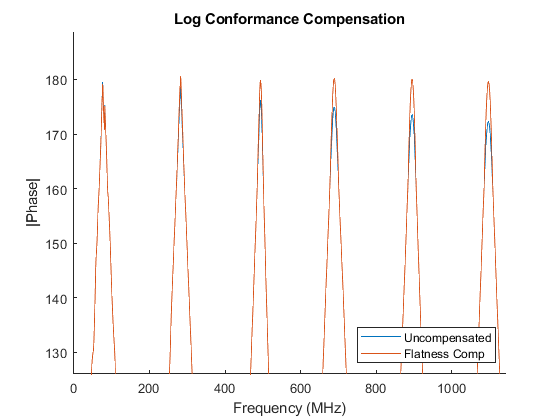
\includegraphics[width=0.8\linewidth]{log_conformance_compensation_zoomed.png}
	\caption{Correction of non idealities of the AD8302 phase detector output}
	\label{fig:phase_comp}
\end{figure}

\subsection{Software Development}
The host software is written in Python which allows the utilisation of numerous libraries, along with being cross platform such that any computer, including small devices such as a Raspberry Pi can be used to control the VNA. It consists of two classes, \texttt{VNA} and \texttt{Plot} which control the interaction with the VNA and calibration, along with plotting and file IO respectively. Due to time constraints a GUI was unable to be designed for the interface, and instead there is a command line interface which enables full control over all required actions. A command parser is utilised to determine what the user would like to do, however unlike on the VNA there are a number of assertions utilised to ensure that the user is only able to select correct values for settings such as frequency span and output power. 

To connect to the VNA, the script searches all connected COM ports and until it finds a device with the expected VID:PID pair as set in firmware. It then sends a \texttt{WHOAMI} command to the VNA, and upon confirmation that it returns the correct value \texttt{Josh's VNA!} it will finalise the connection. The second step is required at the VID:PID pair has been set during development without licencing it from the USB consortium and as such there is the possibility of conflicts if another device is connected with the same ID. 

Commanding the VNA requires composing a string with the required command parameters, sending it over the COM port to the VNA, and awaiting a response. To differentiate the responses between information that the user may want to see printed to console and the data required by the VNA, user information is prefixed with a \texttt{>} and the script will print that line to the user instead of storing it in the arrays used for VNA data. 

S-parameter data is then processed, starting with phase correction and if enabled calibration adjustments, both of which will be discussed below. From there the file is saved to disk as a touchstone file, which is the industry standard format for S-parameter data. The most recent data is stored with a generic file name, however there are commands to save the file with a custom file name, as this not only identifies the file, but can be loaded in later to compare against a second measurement. 

Plotting is achieved by loading the recently saved file and using the methods within scikit-rf to plot in formats such as S-parameter, Smith Chart, phase, and polar measurement, and if implemented there are other options such as group delay and VSWR which can be displayed with ease. Custom plotting options such as \texttt{mag-phase} which utilise the subplot command to show multiple figures at once, along with \texttt{compare} which loads a previously saved touchstone files and allows comparison between them are available which enables easy comprehension of the recorded measurements.  

\subsubsection{Phase Correction}
Phase correction is required as the phase numbers returned from the VNA are absolute in value due to the function of the AD8302 gain and phase detector, and need to be mapped to the +180$^\circ$ to -180$^\circ$ range which exists in the phase domain. Figure \ref{fig:phase_correction} shows an example of the correction, and the key steps in the remapping function are described below:
\begin{itemize}
	\item The raw phase data is smoothed with a running mean low pass filter to remove any high or low outliers which will affect peak detection.
	\item SciPy's \texttt{find\_peaks} method is used on the filtered data to find when the phase has a maxima which corresponds to an absolute value of 180$^\circ$, along with finding valleys which represent a phase value of 0$^\circ$.
	\item The first and last phase values in the series are also determined, as they are required to determine the gradient in the next step. 
	\item The gradient between these key points is determined, and by observation of Figure \ref{fig:ad8302_VPHS_conformance} it can be seen that a positive gradient corresponds to a negative phase, and vice versa. Using this, the phase in the positive sloped segments are inverted, which results in the phase correctly representing the entire +180$^\circ$ to -180$^\circ$ range which is expected for phase measurements. 
\end{itemize} 

\begin{figure}[H]
	\centering
	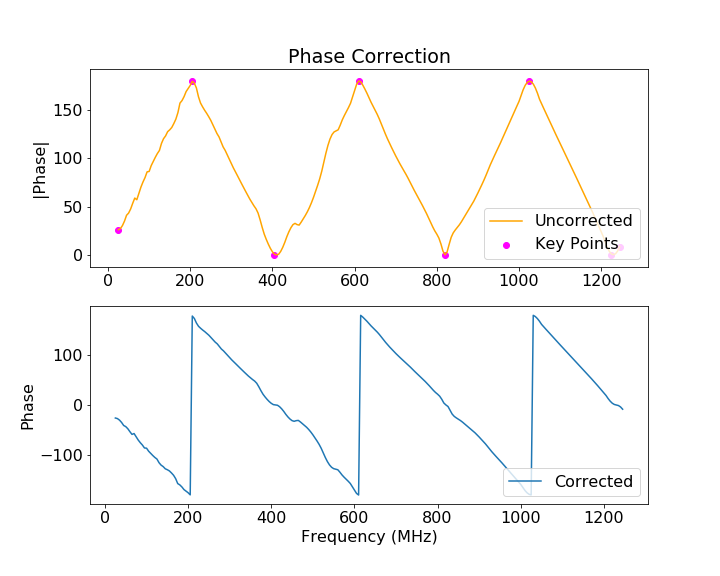
\includegraphics[width=\linewidth]{phase_correction.png}
	\caption{Absolute phase to actual phase correction}
	\label{fig:phase_correction}
\end{figure}


\subsubsection{Calibration}
Calibration is crucial for a VNA as not only does it compensate for non idealities in the VNA, but is able to change the reference plane at which measurements are taken, which allows for the use of cables and de embedding of DUTs on a PCB when the correct test fixtures and standards are used. For a two port VNA, there are six types of systematic errors, \cite{keysight_vna_cal} which are shown in Figure \ref{fig:vna_error}.

When a one port measurement is being taken, the number of possible errors is reduced as port B is no longer being utilised, and as such the transmission tracking, load mismatch, and crosstalk errors are eliminated. For a typical VNA capable of measuring all four S-parameters of a two port device these error terms exists in both the forward and reverse directions, as as such there are twelve error terms. This is where the common twelve term (or SOLT) calibration process results from, as it is a form of vector error correction capable of correcting the systematic errors outlined above. It requires known short, open, load, and through calibration standards, and by measuring those standards it is able to generate an error model which can be used to remove systematic errors from the measurements. 

\begin{figure}[H]
	\centering
	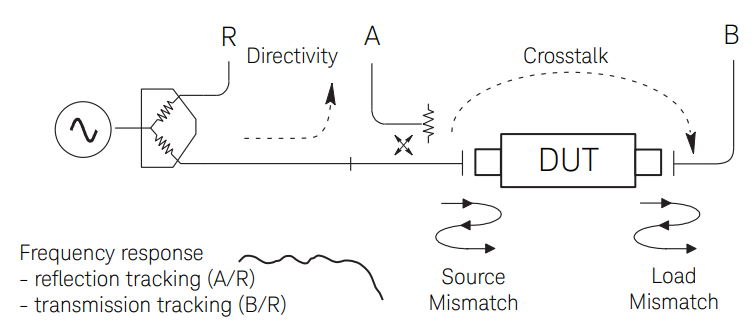
\includegraphics[width=\linewidth]{vna_errors.png}
	\caption{Sources of error in a two port VNA}
	\label{fig:vna_error}
\end{figure}

This was achieved by measuring home-made calibration standards on a commercial VNA, effectively transferring the calibration from the expensive calibration kit to the home-made version. After selecting to calibrate the VNA from the Python CLI, it prompts the user through measuring the required standards, before utilising the inbuilt one port and SOLT calibration methods available in scikit-rf to calculate the error model, which is then applied to future measurements.



